\documentclass[a4paper,11pt]{article}
\usepackage[margin=1in]{geometry}
\usepackage{tikz,tkz-graph,graphicx}
\usepackage{xcolor}
\usepackage{subcaption}

\usetikzlibrary{arrows.meta,positioning,shapes,chains,calc}

\definecolor{lightOrange}{rgb}{0.9921875,0.890625,0.69921875}
\definecolor{darkOrange}{rgb}{0.96875,0.64453125,0.33203125}
\definecolor{skyBlue}{rgb}{0.66796875,0.875,0.97265625}
\definecolor{darkBlue}{rgb}{0.046875,0.69140625,0.9375}

\begin{document}

\section*{Picture}
\begin{figure}[h]
	\centering
	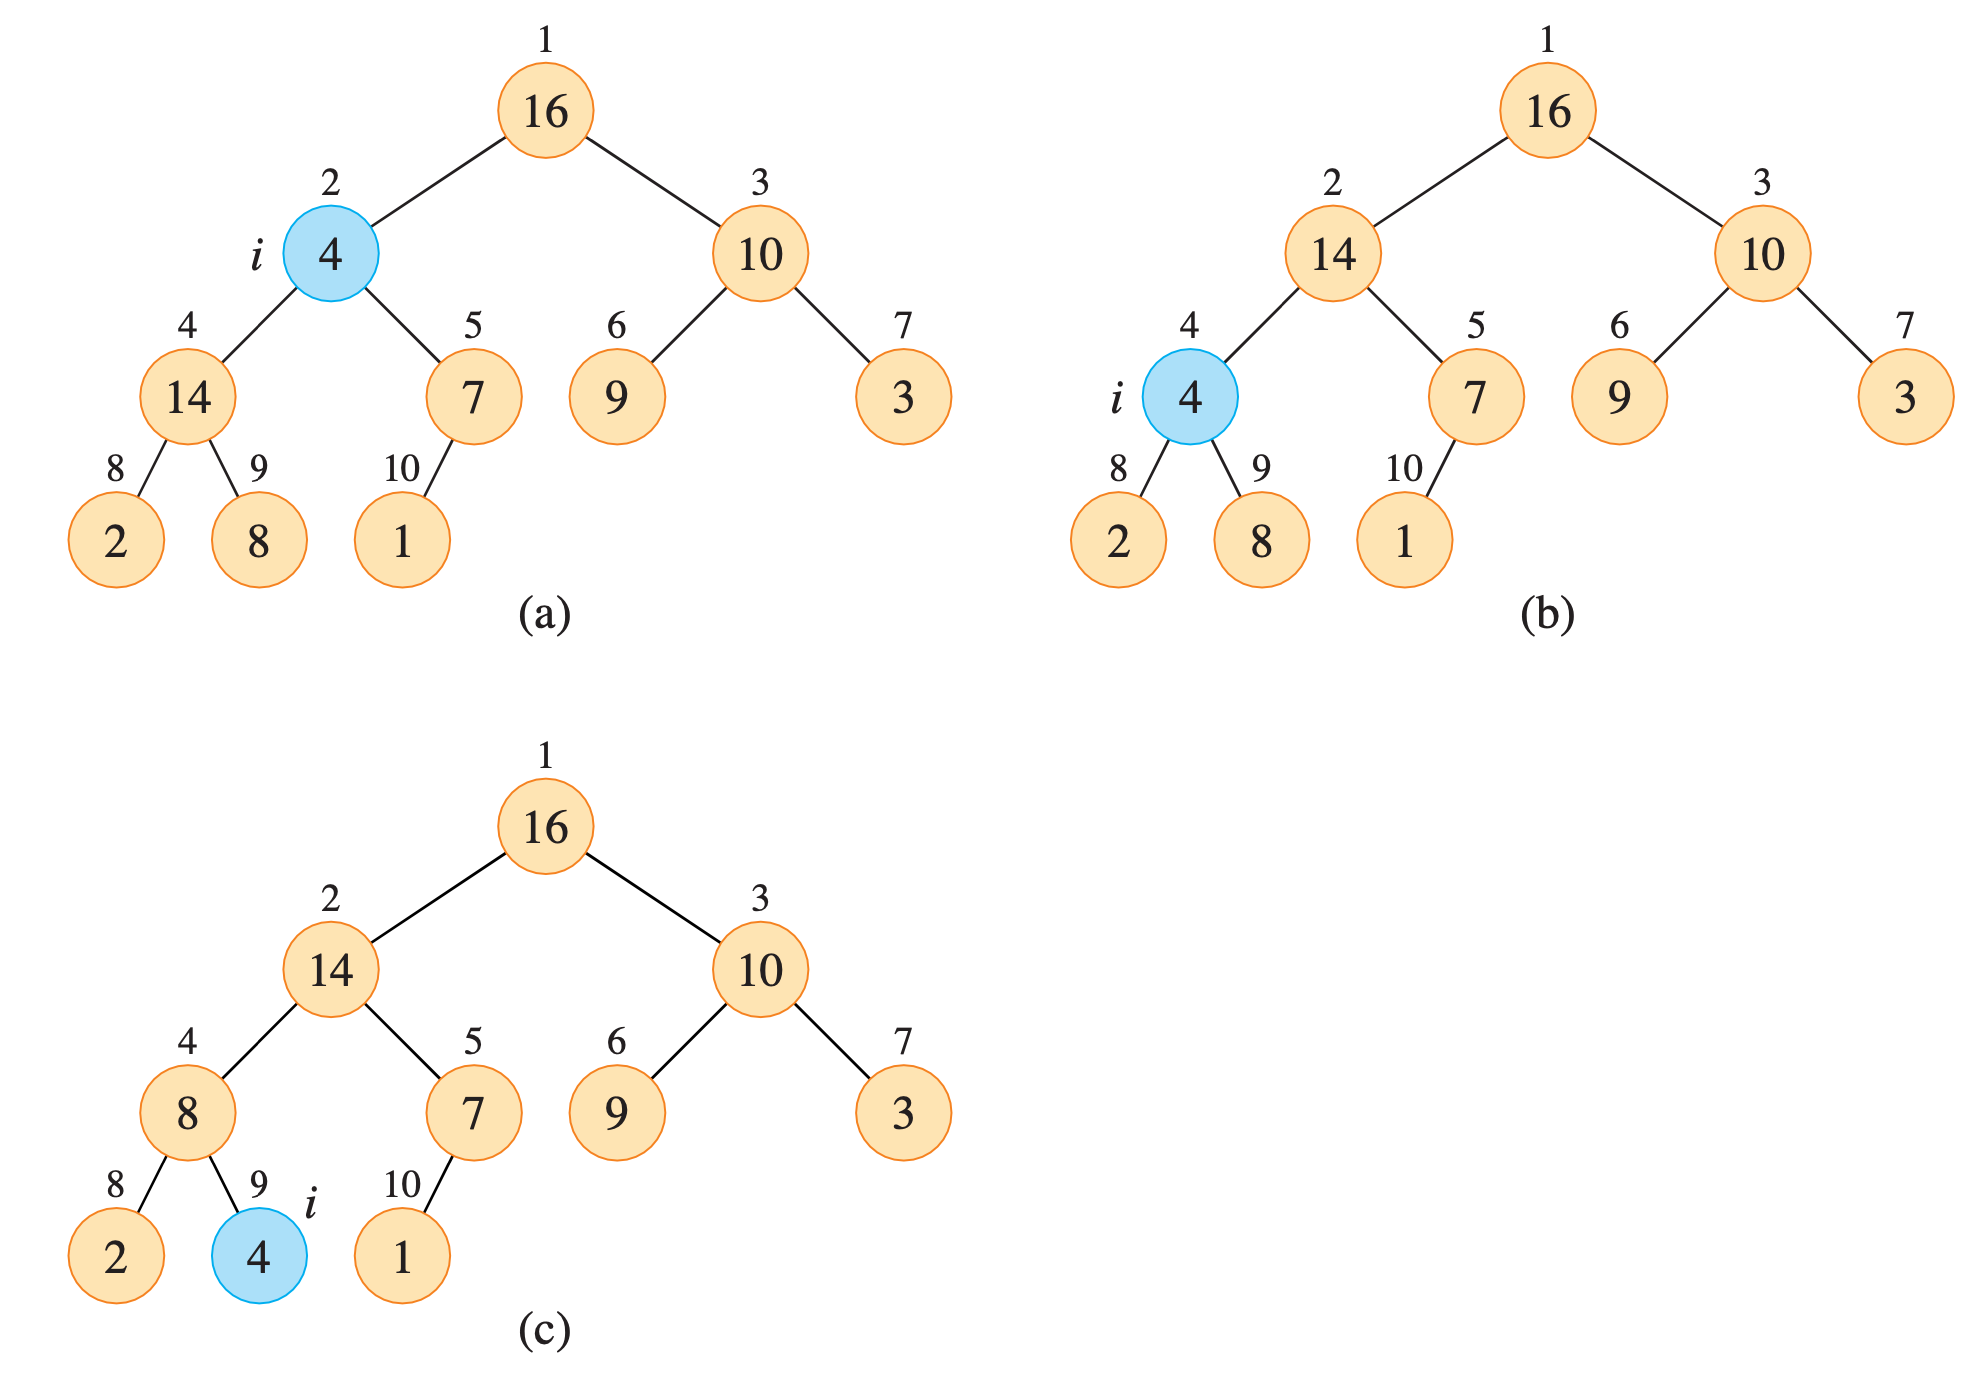
\includegraphics[width=0.7\textwidth]{./4.png}
\end{figure}

\section*{PDF}
\newcommand{\scale}{0.6}
\begin{figure}[h]
  \begin{subfigure}[t]{0.5\textwidth}\vskip 0pt
    \begin{tikzpicture}[%
      scale=\scale,
      level distance=1.75cm,
      sibling distance=1.75cm,
      nodes={
        draw,
        circle,
        color=darkOrange,
        fill=lightOrange,
        text=black,
        inner sep=3pt,
        outer sep=0pt,
        minimum size=3ex
      }
      ]
      
      \tikzset{
        blueNode/.style={
          color=darkBlue,
          fill=skyBlue,
          text=black
        }
      }
      
      \newcommand{\NodeRoot}[2]{\node[label=above:#2]{#1}}
      \newcommand{\Node}[2]{node[label=above:#2]{#1}}
      \newcommand{\NodeBlue}[3]{%
        node[blueNode,label=above:#2,label=#3:$i$]{#1}%
      } 
      
      \NodeRoot{16}{1}
      child {\NodeBlue{4}{2}{left}
        child {\Node{14}{4}
          child {\Node{2}{8}}
          child {\Node{8}{9}}
        }
        child[missing]
        child {\Node{7}{5}
          child {\Node{1}{10}}
          child[missing]
        }
      }
      child[missing]
      child[missing]
      child {\Node{10}{3}
        child {\Node{9}{6}}
        child[missing]
        child {\Node{3}{7}}
      };
    \end{tikzpicture}
    \caption{~}
  \end{subfigure}\hfill\begin{subfigure}[t]{0.5\textwidth}\vskip 0pt
    \begin{tikzpicture}[%
      scale=\scale,
      level distance=1.75cm,
      sibling distance=1.75cm,
      nodes={
        draw,
        circle,
        color=darkOrange,
        fill=lightOrange,
        text=black,
        inner sep=3pt,
        outer sep=0pt,
        minimum size=3ex
      }
      ]
      
      \tikzset{
        blueNode/.style={
          color=darkBlue,
          fill=skyBlue,
          text=black
        }
      }
      
      \newcommand{\NodeRoot}[2]{\node[label=above:#2]{#1}}
      \newcommand{\Node}[2]{node[label=above:#2]{#1}}
      \newcommand{\NodeBlue}[3]{%
        node[blueNode,label=above:#2,label=#3:$i$]{#1}%
      } 
      
      \NodeRoot{16}{1}
      child {\Node{14}{2}
        child {\NodeBlue{4}{2}{left}
          child {\Node{2}{8}}
          child {\Node{8}{9}}
        }
        child[missing]
        child {\Node{7}{5}
          child {\Node{1}{10}}
          child[missing]
        }
      }
      child[missing]
      child[missing]
      child {\Node{10}{3}
        child {\Node{9}{6}}
        child[missing]
        child {\Node{3}{7}}
      };
    \end{tikzpicture}
    \caption{~}
  \end{subfigure}

  \begin{subfigure}[t]{0.5\textwidth}\vskip 0pt
    \begin{tikzpicture}[%
      scale=\scale,
      level distance=1.75cm,
      sibling distance=1.75cm,
      nodes={
        draw,
        circle,
        color=darkOrange,
        fill=lightOrange,
        text=black,
        inner sep=3pt,
        outer sep=0pt,
        minimum size=3ex
      }
      ]
      
      \tikzset{
        blueNode/.style={
          color=darkBlue,
          fill=skyBlue,
          text=black
        }
      }

      \newcommand{\NodeRoot}[2]{\node[label=above:#2]{#1}}
      \newcommand{\Node}[2]{node[label=above:#2]{#1}}
      \newcommand{\NodeBlue}[3]{%
        node[blueNode,label=above:#2,label=#3:$i$]{#1}%
      } 
      
      \NodeRoot{16}{1}
      child {\Node{14}{2}
        child {\Node{8}{2}
          child {\Node{2}{8}}
          child {\NodeBlue{4}{9}{above right}}
        }
        child[missing]
        child {\Node{7}{5}
          child {\Node{1}{10}}
          child[missing]
        }
      }
      child[missing]
      child[missing]
      child {\Node{10}{3}
        child {\Node{9}{6}}
        child[missing]
        child {\Node{3}{7}}
      };
    \end{tikzpicture}
    \caption{~}
  \end{subfigure}
\end{figure}

\end{document}